\lab{Algorithms}{Conjugate-Gradient}{Conjugate-Gradient}
\objective{Learn About the Conjugate-Gradient Algorithm and its Uses}

\section*{Descent Algorithms and the Conjugate-Gradient Method}
There are many possibilities for solving a linear system of equations, each method with its own set of pros and cons. In this lab we
will explore the \emph{Conjugate-Gradient algorithm}, which is a method for solving large systems of equations where other methods,
such as Cholesky factorization and simple Gaussian elimination, are unsuitable. The algorithm, however, works equally well for
optimizing convex quadratic functions, and it can even be extended to more general classes of optimization problems.

The type of linear system that Conjugate-Gradient can solve involves a matrix with special structure.
Given symmetric positive definite $n\times n$ matrix $Q$ and an $n$-vector $b$, we wish to find the vector $x$ satisfying
\[
Qx = b.
\]
A unique solution exists because positive definiteness implies invertibility.
For our purposes here, it is useful to recast this problem as an equivalent optimization problem:
\[
\min_{x} f(x) := \frac{1}{2}x^TQx - b^Tx + c.
\]
Notice that $\nabla f(x) = Qx - b$, so that minimizing $f(x)$ is the same as solving
\[
0 = \nabla f(x) = Qx - b,
\]
and this is our original linear system.

So how do we go about minimizing the quadratic objective function $f$? Line Search methods belonging to the class called
\emph{descent algorithms} use the following strategy: start with an initial guess $x_0$, identify a direction from
this particular point along which the objective function decreases (called a \emph{descent direction}), and perform a line-search to
find a new point $x_1$ satisfying $f(x_1) < f(x_0)$. Continue iteratively to produce a sequence of points $x_0, x_1, x_2, \ldots$
that (hopefully) converges to the true minimizer.

One obvious candidate for the descent direction from some point $x_i$ is simply
$-\nabla f(x_i)$, since this vector points in the direction of steepest decrease. This procedure is known as the Method of Steepest
Descent. Steepest descent, however, can be very inefficient for certain problems: depending on the geometry
of the objective function, the sequence of points can ``zig-zag" back and forth without making appreciable progress toward the true
minimizer. In contrast, the Conjugate-Gradient algorithm ensures that the true global minimizer is reached in at most $n$ steps. See
Figure \ref{basis:steepVsConj} for an illustration of this contrast.
To understand why this is the case and how the algorithm chooses each descent direction, we next discuss the idea of vector conjugacy.

\begin{figure}
\centering
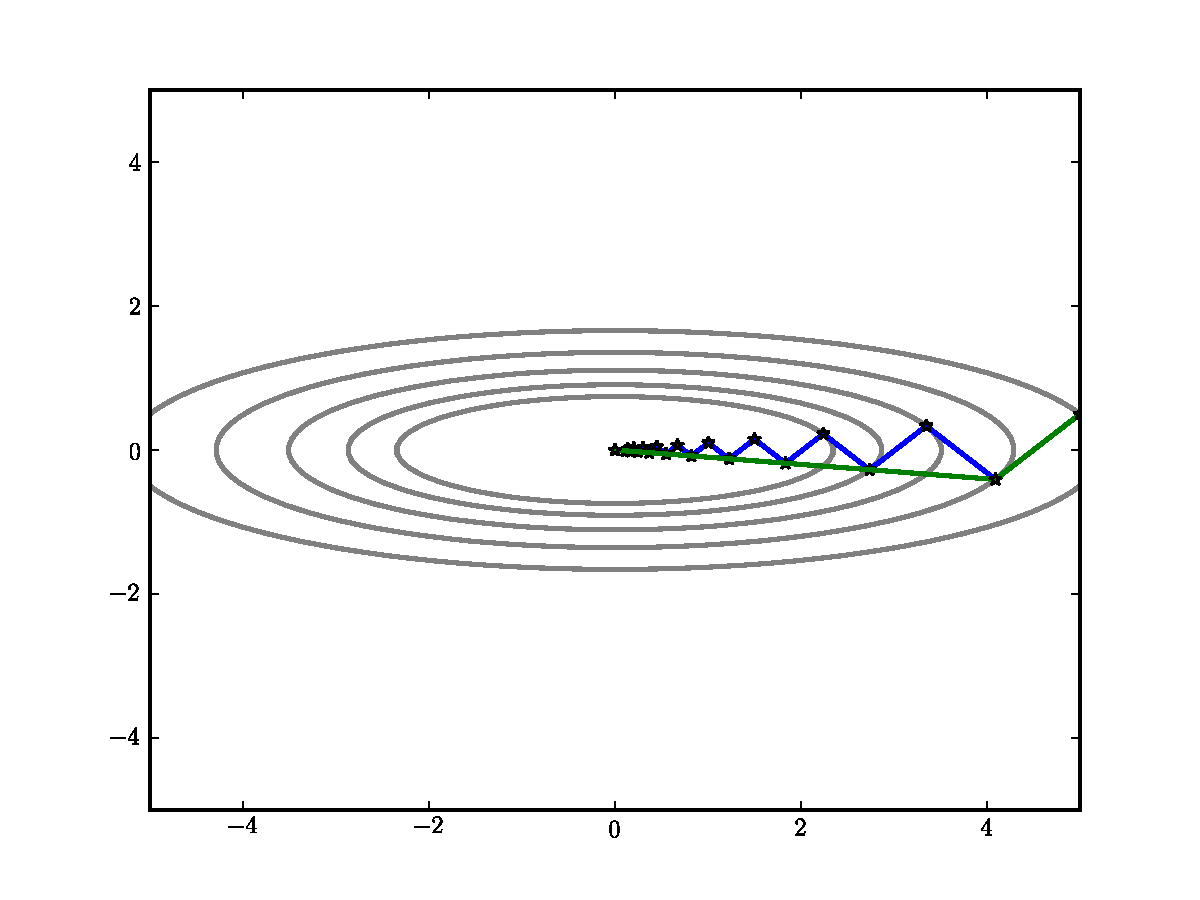
\includegraphics[width=\textwidth]{steepVsConj.pdf}
\caption{Paths traced by Steepest Descent (blue) and Conjugate-Gradient (green). Notice the
zig-zagging nature of the Steepest Descent path, as opposed to the direct Conjugate-Gradient path,
which finds the minimizer in 2 steps.}
\label{basis:steepVsConj}
\end{figure}

\section*{Conjugacy}
Consider again our symmetric positive definite $n \times n$ matrix $Q$. Two vectors $x, y \in \mathbb{R}^n$ are said to be \emph{conjugate}
with respect to $Q$ if $x^TQy = 0$. A set of vectors $\{x_0, x_1, \ldots, x_m\}$ is said to be conjugate if each pair of vectors are conjugate
to each other. Note that if $Q = I$, then conjugacy is the same as orthogonality. Thus, the notion of conjugacy is in some ways a generalization
of orthogonality. It turns out that a conjugate set of vectors is linearly independent, and a conjugate basis--which can be constructed in a manner
analogous to the Gram-Schmidt orthogonalization process--can be used to diagonalize the matrix $Q$.
These are some of the theoretical reasons behind the effectiveness of the Conjugate-Gradient algorithm.
%Take this section out? Add more to it?

\section*{The Algorithm}
If we are given a set of $n$ $Q$-conjugate vectors, we can simply choose these as our direction vectors and follow the basic descent algorithm.
Convergence to the minimizer in at most $n$ steps is guaranteed because each iteration in the algorithm minimizes the objective function
over an expanding affine subspace of dimension equal to the iteration number. Thus, at the $n$-th iteration, we have minimized the function over all of
$\mathbb{R}^n$.

Unfortunately, we are not often given a set of conjugate vectors in advance, so how do we produce such a set? As mentioned earlier, a
Gram-Schmidt process could be used, and the set of eigenvectors also works, but both of these options are computationally expensive.
Built into the algorithm is a way to determine a new conjugate direction based only on the previous direction, which means less memory usage and
faster computation. We have stated the details of Conjugate-Gradient in Algorithm \ref{alg:conjgrad}.
\begin{algorithm}
\begin{algorithmic}[1]
\Procedure{Conjugate-Gradient Algorithm}{}
    \State \textrm{Choose initial point } $x_0$.
    \State $r_0 \gets Qx_0 - b, d_0 \gets -r_0, k \gets 0$.
    \While{$r_k \neq 0$}
        \State $\alpha_k \gets \frac{r_k^Tr_k}{d_k^TQd_k}$.
        \State $x_{k+1} \gets x_k + \alpha_kd_k$.
        \State $r_{k+1} \gets r_k + \alpha_kQd_k$.
        \State $\beta_{k+1} \gets \frac{r_{k+1}^Tr_{k+1}}{r_k^Tr_k}$.
        \State $d_{k+1} \gets -r_{k+1} + \beta_{k+1}d_k$.
        \State $k \gets k+1$.
    \EndWhile
\EndProcedure
\end{algorithmic}
\caption{Conjugate-Gradient Algorithm}
\label{alg:conjgrad}
\end{algorithm}

Note that the points $x_i$ are the successive approximations to the minimizer, the vectors $d_i$ are the conjugate descent
directions, and the vectors $r_i$, which actually correspond to the steepest descent directions, are used in determining the conjugate directions.
The constants $\alpha_i$ and $\beta_i$ are used in the line-search and in ensuring the $Q$-conjugacy of the descent directions, respectively.

The most numerically expensive computation in the algorithm is matrix-vector multiplication.
Notice, however, that each iteration of the algorithm only requires one distinct matrix-vector multiplication, $Qd_k$. The rest of the
operations are simply vector-vector multiplication, addition, and scalar multiplication. This makes for a very fast algorithm.
As noted earlier, Conjugate-Gradient is especially preferred when $Q$ is large and sparse. In this case, it may be possible to
design a specialized sub-routine that performs matrix-vector multiplication by $Q$, taking advantage of its sparseness. Doing so may
lead to further speed-ups in the overall algorithm.

We now have an algorithm that can solve certain $n \times n$ linear systems and minimize quadratic functions on $\mathbb{R}^n$ in at most $n$ steps,
and sometimes fewer, depending on the spectrum of the matrix $Q$. Further improvements on convergence may be obtained by preconditioning the matrix,
but we do not go into detail here.

\begin{problem}
Implement the basic Conjugate-Gradient algorithm presented above. Write a function \li{conjugateGradient} that accepts a vector $b$, an initial
guess $x_0$, and a callable function
object that performs matrix-vector multiplication by a symmetric positive-definite matrix $Q$ as inputs.
Return the solution $x^*$ to the linear system $Qx = b$, using the Conjugate-Gradient algorithm.
\end{problem}

\section*{Example}
We now work through an example that demonstrates the usage of the Conjugate-Gradient algorithm. We assume that we have already written
the specified function in the above problem.

We must first generate a symmetric positive definite matrix $Q$. This can be done by generating a random matrix $A$ and setting $Q = A^TA$.
So long as $A$ is of full column rank, the matrix $Q$ will be symmetric positive definite.
\begin{lstlisting}
>>> import numpy as np
>>> from scipy import linalg as la

>>> # initialize the desired dimension of the space
>>> n = 10

>>> # generate Q, b
>>> A = np.random.random((n,n))
>>> Q = A.T.dot(A)
>>> b = np.random.random(n)
\end{lstlisting}
At this point, check to make sure that $Q$ is nonsingular by examining its determinant (use \li{scipy.linalg.det}).
Provided that the determinant is nonzero, we proceed by writing a function that performs matrix-vector multiplication by $Q$ (we
will not take advantage of sparseness just now), randomly selecting a starting point (Conjugate-Gradient is not sensitive to the location of
the starting point), obtaining the answer using our function, and checking it with the answer obtained by \li{scipy.linalg.solve}.
\begin{lstlisting}
>>> def mult(x):
>>>     return Q.dot(x)

>>> # generate random starting point
>>> x0 = np.random.random(n)

>>> # find the solution
>>> x = conjugateGradient(b, x0, mult)

>>> # compare to the answer obtained by SciPy
>>> print np.allclose(x, la.solve(Q,b))
\end{lstlisting}
The output of that last print statement should be \li{True}.

Time the performance of your algorithm and of \li{scipy.linalg.solve} on inputs of size 100.

\section*{Application: Least Squares and Linear Regression}
The Conjugate-Gradient method can be used to solve linear least squares problems, which are ubiquitous in applied science.
Recall the least squares problem can be formulated as an optimization problem:
\[
\min_x \|Ax - b\|_2,
\]
where $A$ is an $m \times n$ matrix with full column rank, $x \in \mathbb{R}^n$, and $b \in \mathbb{R}^m$. The solution can
be calculated analytically, given by
\[
x^* = (A^TA)^{-1}A^Tb,
\]
or in other words, the minimizer solves the linear system
\[
A^TAx = A^Tb.
\]
Since $A$ has full column rank, we know that $A^TA$ is an $n \times n$ matrix of rank $n$, which means it is invertible. We can
therefore conclude that $A^TA$ is symmetric positive definite, so we may use Conjugate-Gradient to solve the linear system
and obtain the least squares solution.

Linear least squares is the mathematical underpinning of linear regression, a very common technique in many scientific fields.
In a typical linear regression problem, we have a set of real-valued data points $y_1,\ldots, y_m$, where each
$y_i$ is paired with a corresponding set of predictor variables $x_{i,1}, x_{i,2}, \ldots, x_{i,n}$ with $m > n$.
The linear regression model posits that
\[
y_i = \beta_0 + \beta_1x_{i,1} + \beta_2x_{i,2} + \cdots + \beta_nx_{i,n} + \epsilon_i
\]
for $i = 1, 2, \ldots, m$. The real numbers $\beta_0,\ldots,\beta_n$ are known as the parameters of the model, and the
$\epsilon_i$ are independent normally-distributed error terms. Our task is to calculate the parameters that best fit the data.
This can be accomplished by posing the problem in terms of linear least squares: define
\[
b = [y_1, \ldots, y_m]^T,
\]
\[
A =
\begin{bmatrix}
1 & x_{1,1} & x_{1,2} & \cdots & x_{1,n}\\
1 & x_{2,1} & x_{2,2} & \cdots & x_{2,n}\\
\vdots & \vdots & \vdots & \ddots & \vdots\\
1 & x_{m,1} & x_{m,2} & \cdots & x_{m,n}
\end{bmatrix},
\]
and
\[
x = [\beta_0, \beta_1,\ldots, \beta_n]^T.
\]
Now use Conjugate-Gradient to solve the system
\[
A^TAx = A^Tb.
\]
The solution $x^* = [\beta_0^*, \beta_1^*, \ldots, \beta_n^*]^T$ gives the parameters that best fit the data.
These values can be understood as defining the hyperplane that best fits the data. See Figure \ref{fig:linregression}.

\begin{figure}
\centering
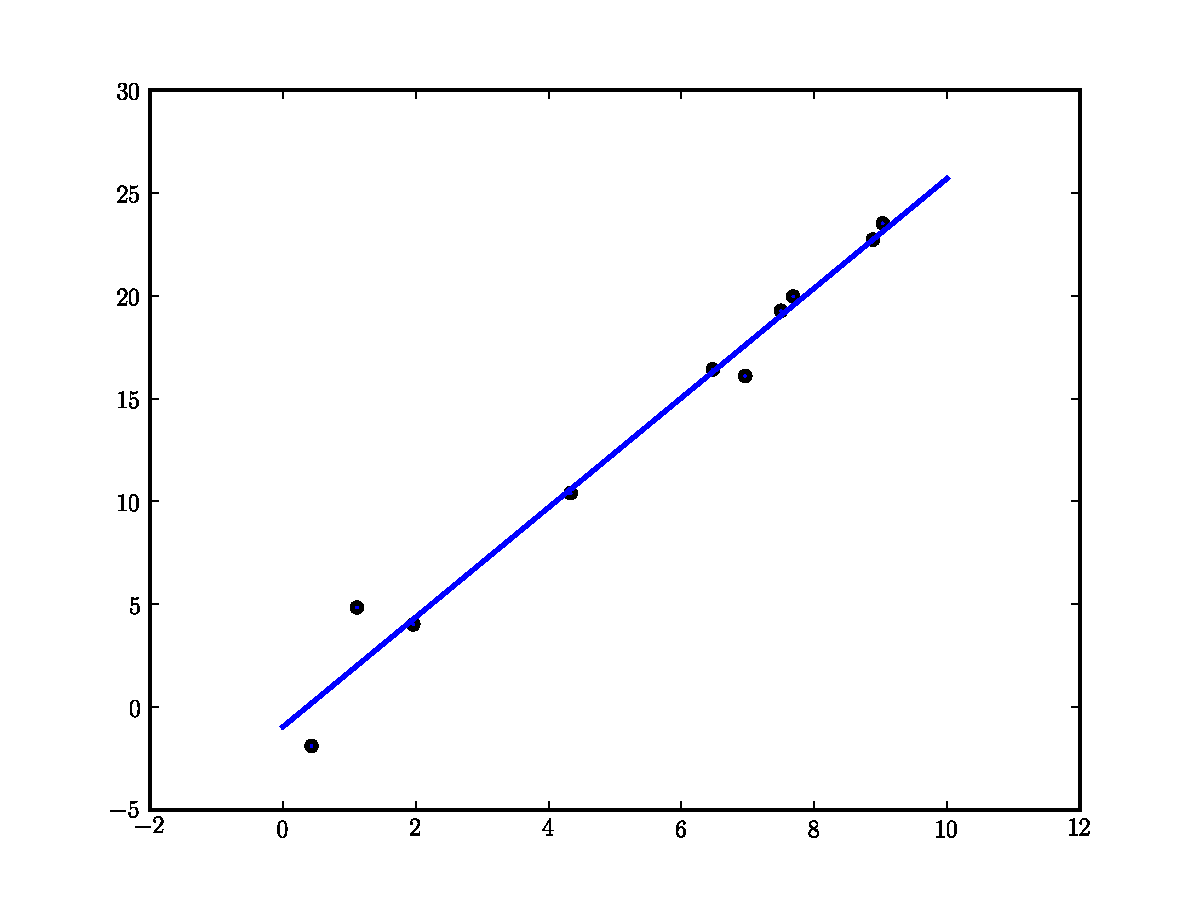
\includegraphics[width=\textwidth]{linregression.pdf}
\caption{Solving the Linear Regression problem results in a best-fit hyperplane.}
\label{fig:linregression}
\end{figure}

\begin{problem}
Using your Conjugate-Gradient function, solve the linear regression problem specified by the data file
\li{linregression.txt}. This is a whitespace-delimited text file formatted so that the $i$-th row consists of
$y_i, x_{i,1}, \ldots, x_{i,n}$. Use the function \li{numpy.loadtxt} to load in the data. Report your solution.
\end{problem}

\section*{Non-linear Conjugate-Gradient Algorithms}
The algorithm presented above is only valid for certain linear systems and quadratic functions, but the basic strategy may be adapted
to minimize more general convex or non-linear functions. There are multiple ways to modify the algorithm, and they all involve getting
rid of $Q$, since there is no such $Q$ for non-quadratic functions. Generally speaking, we need to find new formulas for the $\alpha_k$,
$r_k$, and $\beta_k$.

The scalar $\alpha_k$ is simply the result of performing a line-search in the given direction $d_k$, so we may define
\[
\alpha_k = \underset{x}{\arg\min}f(x_k + \alpha d_k).
\]
The vector $r_k$ in the original algorithm was really just the gradient of the objective
function, and so we may define 
\[
r_k = \nabla f(x_k).
\]
There are various ways to define the constants $\beta_k$ in this more general setting, and the
right choice will depend on the nature of the objective function. A well-known formula, due to Fletcher and Reeves, is
\[
\beta_{k+1} = \frac{\nabla f_{k+1}^T \nabla f_{k+1}}{\nabla f_{k}^T \nabla f_{k}}.
\]

Making these adjustments is not difficult, but we will opt instead to use built-in functions in Python. In particular,
the SciPy module \li{scipy.optimize} provides a function \li{fmin_cg}, which uses a non-linear Conjugate-Gradient method
to minimize general functions. Using this function is easy -- we only need to pass to it the objective function and an
initial guess.

\section*{Application: Logistic Regression}
Logistic regression is an important technique in statistical analysis and classification. The core problem in
logistic regression involves an optimization that we can tackle using nonlinear Conjugate-Gradient.

As in linear regression, we have a set of data points $y_i$ together with predictor variables
$x_{i,1}, x_{i,2}, \ldots, x_{i,n}$ for $i = 1, \ldots, m$. However, the $y_i$ are binary data points --
that is, they are either $0$ or $1$. Furthermore, instead of having a linear relationship between the
data points and the response variables, we assume the following probabilistic relationship:
\[
\mathbb{P}(y_i = 1 \, | \, x_{i,1}, \ldots, x_{i,n}) = p_i,
\]
where
\[
p_i = \frac{1}{1+\exp(-(\beta_0 + \beta_1x_{i,1} + \cdots + \beta_nx_{i,n}))}.
\]
The parameters of the model are the real numbers $\beta_0, \beta_1,\ldots, \beta_n$.
Observe that we have $p_i \in (0, 1)$ no matter the values of the predictor variables and parameters.

The probability of observing the data points $y_i$ under this model, assuming they are independent, is given by
the expression
\[
\prod_{i=1}^m p_i^{y_i}(1-p_i)^{1-y_i}.
\]
We seek to choose the parameters $\beta_0, \ldots, \beta_n$ that maximize this probability.
To this end, define the \emph{likelihood function} $L:\mathbb{R}^{n+1} \rightarrow \mathbb{R}$ by
\[
L(\beta_0, \ldots, \beta_n) = \prod_{i=1}^m p_i^{y_i}(1-p_i)^{1-y_i}.
\]
We can now state our core problem as follows:
\[
\max_{(\beta_0,\ldots,\beta_n)}L(\beta_0, \ldots, \beta_n).
\]

Maximizing this function can be problematic for numerical reasons. By taking the logarithm of the likelihood,
we have a more suitable objective function whose maximizer agrees with that of the original likelihood function,
since the logarithm is strictly monotone increasing. Thus, we define the \emph{log-likelihood function}
$l : \mathbb{R}^{n+1} \rightarrow \mathbb{R}$ by $l = \log \circ L$.

Finally, we multiply by $-1$ to turn our problem into minimization. The final statement of the problem is:
\[
\min_{(\beta_0,\ldots,\beta_n)}-l(\beta_0, \ldots, \beta_n).
\]
A few lines of calculation reveal that
\begin{align*}
l(\beta_0,\ldots,\beta_n) = &-\sum_{i=1}^{m}\log(1+\exp(-(\beta_0 + \beta_1x_{i,1} + \cdots +\beta_nx_{i,n}))) +\\
 &\sum_{i=1}^m y_i(\beta_0 + \beta_1x_{i,1} + \cdots + \beta_nx_{i,n}).
\end{align*}
The values for the parameters that we obtain are known collectively as the \emph{maximum likelihood estimate}.

Let's work through a simple example. We will deal with just one predictor variable, and therefore two parameters.
The data are given in Table \ref{table:data}.
This is obviously just toy data with no meaning, but one can think of the $y_i$ data points as indicating, for example, the
presence of absence of a particular disease in subject $i$, with $x_i$ being the subject's weight, or age, or something
of the sort.

\begin{table}
  \caption{Data for Logistic Regression Example}
  \centering
  \begin{tabular}{c c}
    \hline\hline
    $y$ & $x$\\
    \hline
    0 & 1 \\
    0 & 2 \\
    0 & 3 \\
    0 & 4 \\
    1 & 5 \\
    0 & 6 \\
    1 & 7 \\
    0 & 8 \\
    1 & 9 \\
    1 & 10\\
    \hline
  \end{tabular}
  \label{table:data}
\end{table}

In the code below we initialize our data.
\begin{lstlisting}
>>> y = np.array([0, 0, 0, 0, 1, 0, 1, 0, 1, 1])
>>> x = np.ones((10, 2))
>>> x[:,1] = np.array([1, 2, 3, 4, 5, 6, 7, 8, 9, 10])
\end{lstlisting}
Although we have just one predictor variable, we initialized \li{x} with two columns,
the first of which consists entirely of ones, and the second of which contains the values of the
predictor variable. This extra column of ones corresponds to the parameter $\beta_0$, which as you
will note is not multiplied by any of the predictor variables in the log-likelihood function.

We next need to write a Python function that returns the value of our objective function for any value of the parameters,
$(\beta_0, \beta_1)$.
\begin{lstlisting}
>>> def objective(b):
>>>     #Return -1*l(b[0], b[1]), where l is the log likelihood.
>>>     return (np.log(1+np.exp(x.dot(b))) - y*(x.dot(b))).sum()
\end{lstlisting}

Finally, we minimize the objective function using \li{fmin_cg}.
\begin{lstlisting}
>>> guess = np.array([1., 1.])
>>> b = fmin_cg(objective, guess)
Optimization terminated successfully.
         Current function value: 4.310122
         Iterations: 13
         Function evaluations: 128
         Gradient evaluations: 32
>>> print b
[-4.35776886  0.66220658]
\end{lstlisting}

We can visualize our answer by plotting the data together with the function
\[
\phi(x) = \frac{1}{1 + \exp(-\beta_0 - \beta_1x)},
\]
using the values $\beta_0, \beta_1$ that we obtained from the minimization.
\begin{lstlisting}
>>> dom = np.linspace(0, 11, 100)
>>> plt.plot(x, y, 'o')
>>> plt.plot(dom, 1./(1+np.exp(-b[0]-b[1]*dom)))
>>> plt.show()
\end{lstlisting}

We obtain the plot in Figure \ref{conj:logreg}. Note that the graph of $\phi$, known as a \emph{sigmoidal curve},
gives the probability of $y$ taking the value $1$ at a particular value of $x$. Observe that as $x$ increases,
this probability approaches $1$. This is reflected in the data.
\begin{figure}
\centering
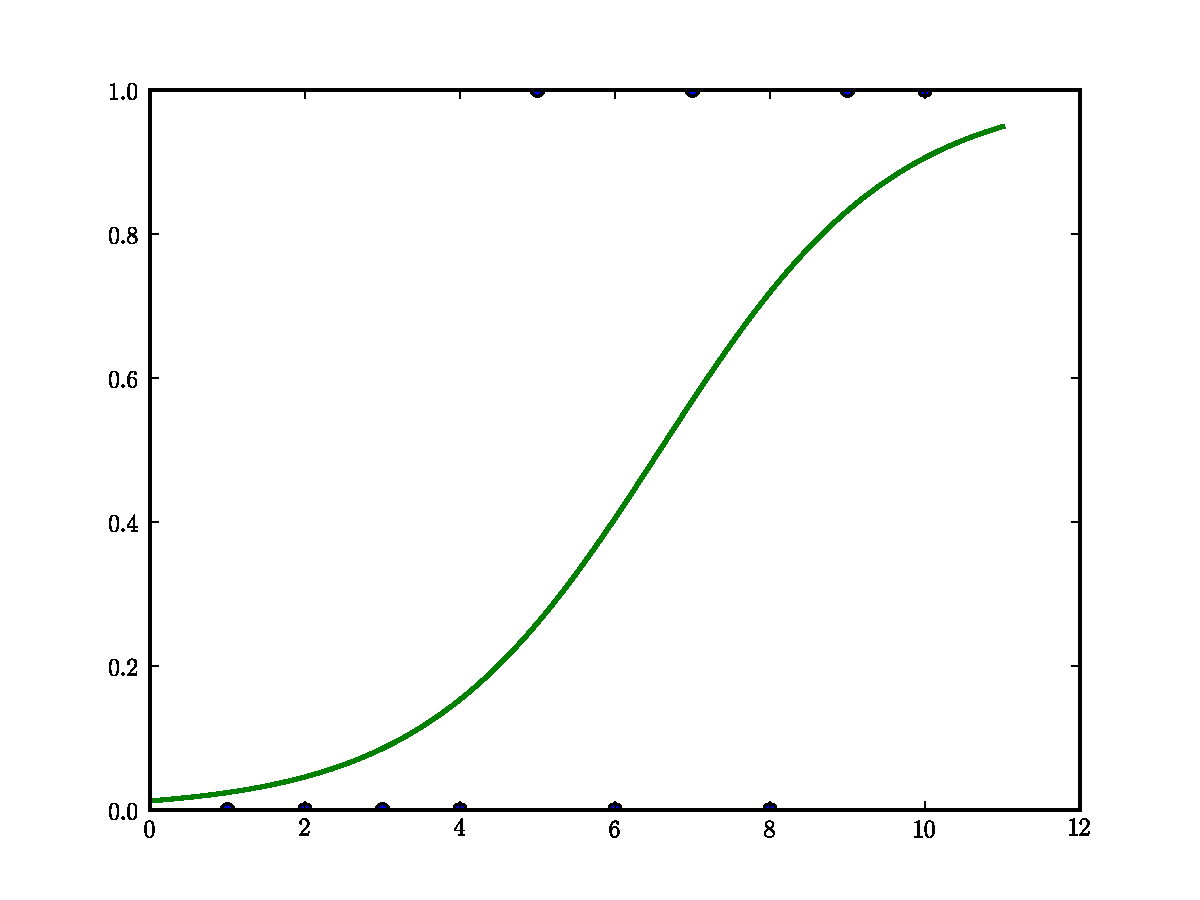
\includegraphics[width=\textwidth]{logreg.pdf}
\caption{Data from the logistic regression example together with the calculated
sigmoidal curve.}
\label{conj:logreg}
\end{figure}

\begin{problem}
Following along with the example given above, find the maximum likelihood estimate of the parameters for
the logistic regression data in the file \li{logregression.txt}. This is a whitespace-delimited text file
formatted so that the $i$-th row consists of $y_i, x_{i,1}, x_{i,2}, x_{i,3}.$ Since there are three
predictor variables, there are four parameters in the model. Report the calculated values.

You should be able to use much of the code above unchanged. In particular, the function \li{objective} does
not need any changes. You simply need to set your variables \li{y} and \li{x} appropriately, and
choose a new initial guess (an array of length four). Note that \li{x} should be an $m \times 4$ array whose first
column consists entirely of ones, whose second column contains the values in the second column of the data file,
and so forth.
\end{problem}

Logistic regression can become a bit more tricky when some of the predictor variables take on binary or categorical
values. In such situations, the data require a bit of pre-processing before running the minimization.

The values of the parameters that we obtained can be useful in analyzing relationships
between the predictor variables and the $y_i$ data points. They can also be used to classify or predict values of new
data points.

%should I give the Polak-Ribi\`{e}, Fletcher-Reeves, and Hestenes-Stiefel formulas? Maybe in the exercises? Should I
%include a discussion of when each choice is appropriate?




